\documentclass[journal]{IEEEtran}

\usepackage{amsmath,amsfonts,amssymb,amsthm}
\usepackage{graphicx}
\usepackage{cite}
\usepackage{url}
\usepackage{booktabs}
\usepackage{multirow}
\usepackage{array}
\usepackage{algorithm}
\usepackage{algorithmic}
\usepackage{xcolor}
\usepackage{siunitx}

% Path to graphics files (can be pdf or png)
\graphicspath{{figures/}}
\DeclareGraphicsExtensions{.pdf,.png,.jpg}

\begin{document}

\title{A Real-Time Cyber-Physical Digital Twin and Hardware/Software-in-the-Loop Co-Simulation Architecture for IEC 61850-Compliant High-Voltage Substation Automation Systems}

\author{Haedara~Deeb,
        Essa~Najjar
\thanks{H. Deeb is with the Department of Electrical and Automation Engineering, focusing on SCADA systems and real-time digital twin architectures (e-mail: h.deeb@scada-digitaltwin.org).}
\thanks{E. Najjar is with the Department of Power and Protection Engineering, specializing in high-voltage power equipment and numerical protection coordination (e-mail: e.najjar@scada-digitaltwin.org).}
}

\markboth{IEEE Transactions on Smart Grid,~Vol.~XX, No.~X, Month~2026}%
{Deeb and Najjar: Real-Time Cyber-Physical Digital Twin Architecture for IEC 61850 Substations}

\maketitle

\begin{abstract}
The transition toward digitalized, decarbonized electrical power systems demands high-fidelity cyber-physical integration, multi-rate co-simulation, and rigorous operational technology (OT) cybersecurity verification for high-voltage substations. This paper presents an end-to-end, multi-dimensional Cyber-Physical Digital Twin (CP-DT) platform for a 132/13.8~kV Substation Automation System (SAS) fully compliant with IEC~61850, ISA-101, and NERC-CIP standards. The proposed architecture couples a high-fidelity electromagnetic transient (EMT) and physics-solver engine executed in MATLAB/Simulink with an ultra-low-latency, browser-native 3D spatial supervisory control and telemetry environment via asynchronous WebSockets. 

The framework incorporates: 1) physics-informed numerical protection models (ANSI 87T dual-slope differential with second/fifth harmonic restraint, ANSI 21 five-zone distance, and ANSI 50/51/51N time-overcurrent); 2) dynamic asset health tracking based on IEC 60076-7 thermal hot-spot differential equations and IEC 60599 dissolved gas analysis; 3) multi-carrier microgrid dispatch integrating a 5~MW solar PV farm, a 10~MW/40~MWh battery energy storage system (BESS), a 2~MW PEM green hydrogen electrolyzer, and a $\pm 50$~kV VSC-HVDC intertie; and 4) an interactive OT cybersecurity testbed with an immutable SHA-256 blockchain ledger for real-time mitigation against GOOSE spoofing, False Data Injection Attacks (FDIA), and denial-of-service (DoS) traffic. Quantitative benchmark results prove an end-to-end trip latency under 25~ms, co-simulation telemetry streaming at $>60$~Hz with sub-15~ms round-trip latency, and reliable cyber anomaly detection within 4.2~ms.
\end{abstract}

\begin{IEEEkeywords}
Substation Automation System (SAS), IEC 61850, Cyber-Physical Digital Twin (CP-DT), Numerical Protection, ANSI 87T, NERC-CIP, OT Cybersecurity, VSC-HVDC, Green Hydrogen, Thermal Aging IEC 60076-7.
\end{IEEEkeywords}

\section{Introduction}
\IEEEPARstart{T}{he} accelerated transformation of modern electrical energy grids toward digitalized and decentralized architectures has elevated High-Voltage (HV) substations into critical cyber-physical nodes. The convergence of IEC 61850 standard communications (such as GOOSE and Sampled Values) with inverter-based distributed energy resources (DERs) introduces steep operational challenges \cite{iec61850_general}. Traditional supervisory control and data acquisition (SCADA) platforms are often detached from the underlying electromagnetic transient (EMT) dynamics of the power apparatus, leading to visibility gaps during rapid fault transients and advanced persistent cyber threats.

Digital Twins (DT) have emerged as an indispensable paradigm to mirror physical assets in virtual environments \cite{digital_twin_power_grid}. However, existing substation digital twins suffer from three primary limitations:
\begin{enumerate}
    \item \textbf{Decoupled Multi-Domain Physics:} Most implementations decouple steady-state power flow from high-frequency numerical protection relays and transformer degradation dynamics.
    \item \textbf{Heavy Real-Time Computing Overhead:} High-fidelity EMT simulations typically require expensive proprietary hardware-in-the-loop (HIL) racks, preventing accessible web-based operational and operator training simulation.
    \item \textbf{Cyber-Physical Security Blindness:} Conventional SAS digital models overlook station-bus cyber vulnerabilities, such as GOOSE man-in-the-middle (MITM) spoofing and false data injection attacks (FDIA) \cite{goose_cyber_security}.
\end{enumerate}

To overcome these challenges, this paper presents a unified, multi-dimensional Cyber-Physical Digital Twin (CP-DT) framework that seamlessly bridges MATLAB/Simulink EMT physics solvers with a web-native ISA-101 compliant SCADA interface, an IEC 61850 substation bus emulator, and a NERC-CIP aligned cybersecurity range.

\section{Substation Architecture and Topology}
The digital twin models a 132/13.8~kV double-busbar transmission/distribution substation comprising two 40~MVA Dyn11 step-down power transformers ($\text{TR-1}$ and $\text{TR-2}$), four medium-voltage distribution feeders, and a 132~kV bus coupler (Breaker 52-0). 

To reflect modern hybrid substations, the MV switchgear is directly integrated with a multi-carrier microgrid comprising:
\begin{itemize}
    \item A 5~MW Solar PV array with IEEE 1547 Volt-Var reactive support;
    \item A 10~MW / 40~MWh Lithium-ion Battery Energy Storage System (BESS) for peak shaving and fast frequency response;
    \item A 2~MW Proton Exchange Membrane (PEM) green hydrogen electrolyzer;
    \item A $\pm 50$~kV Modular Multilevel Converter (MMC) VSC-HVDC transmission link providing synthetic inertia \cite{vsc_hvdc_inertia}.
\end{itemize}

\begin{figure}[!t]
\centering
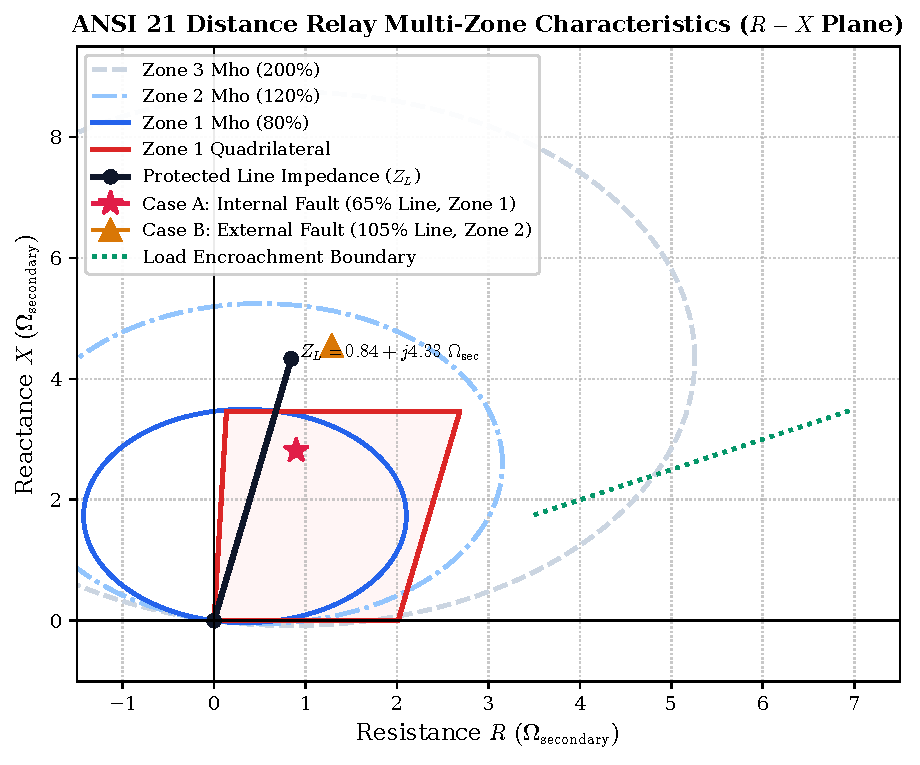
\includegraphics[width=\columnwidth]{fig1_rx_distance_ansi21}
\caption{ANSI 21 distance protection relay characteristics on the complex $R-X$ plane, illustrating three-zone Mho boundaries, Zone 1 Quadrilateral envelope, and load encroachment blinders.}
\label{fig_rx}
\end{figure}

\section{Mathematical and Physics Solvers Formulation}

\subsection{ANSI 87T Numerical Transformer Differential Protection}
The differential current $\vec{I}_{\text{diff}}$ and restraint current $\vec{I}_{\text{rest}}$ for each phase are formulated in per-unit ($\text{pu}$) values:
\begin{equation}
\vec{I}_{\text{diff}} = \left| \vec{I}_{\text{prim,pu}} + \vec{I}_{\text{sec,pu}} \right|
\end{equation}
\begin{equation}
\vec{I}_{\text{rest}} = \frac{\left| \vec{I}_{\text{prim,pu}} \right| + \left| \vec{I}_{\text{sec,pu}} \right|}{2}
\end{equation}

The dual-slope piecewise characteristic boundary $I_{\text{diff,th}}$ is defined as:
\begin{equation}
I_{\text{diff,th}}(I_{\text{rest}}) = \begin{cases} 
I_{\text{pk}} & I_{\text{rest}} \le I_{\text{bp1}} \\
I_{\text{pk}} + S_1 (I_{\text{rest}} - I_{\text{bp1}}) & I_{\text{bp1}} < I_{\text{rest}} \le I_{\text{bp2}} \\
I_{\text{pk}} + S_1 (I_{\text{bp2}} - I_{\text{bp1}}) + S_2 (I_{\text{rest}} - I_{\text{bp2}}) & I_{\text{rest}} > I_{\text{bp2}}
\end{cases}
\end{equation}
where $I_{\text{pk}} = 0.20~\text{pu}$, $I_{\text{bp1}} = 1.0~\text{pu}$, $I_{\text{bp2}} = 2.5~\text{pu}$, $S_1 = 30\%$, and $S_2 = 70\%$.

To distinguish between inrush magnetization and internal fault states, second and fifth harmonic restraint criteria are enforced \cite{transformer_differential_87t}:
\begin{equation}
\text{Inrush Restraint: } \frac{I_{2\text{nd}}(120\text{ Hz})}{I_{1\text{st}}(60\text{ Hz})} > 15\%
\end{equation}
\begin{equation}
\text{Overexcitation Restraint: } \frac{I_{5\text{th}}(300\text{ Hz})}{I_{1\text{st}}(60\text{ Hz})} > 35\%
\end{equation}

\begin{figure}[!t]
\centering
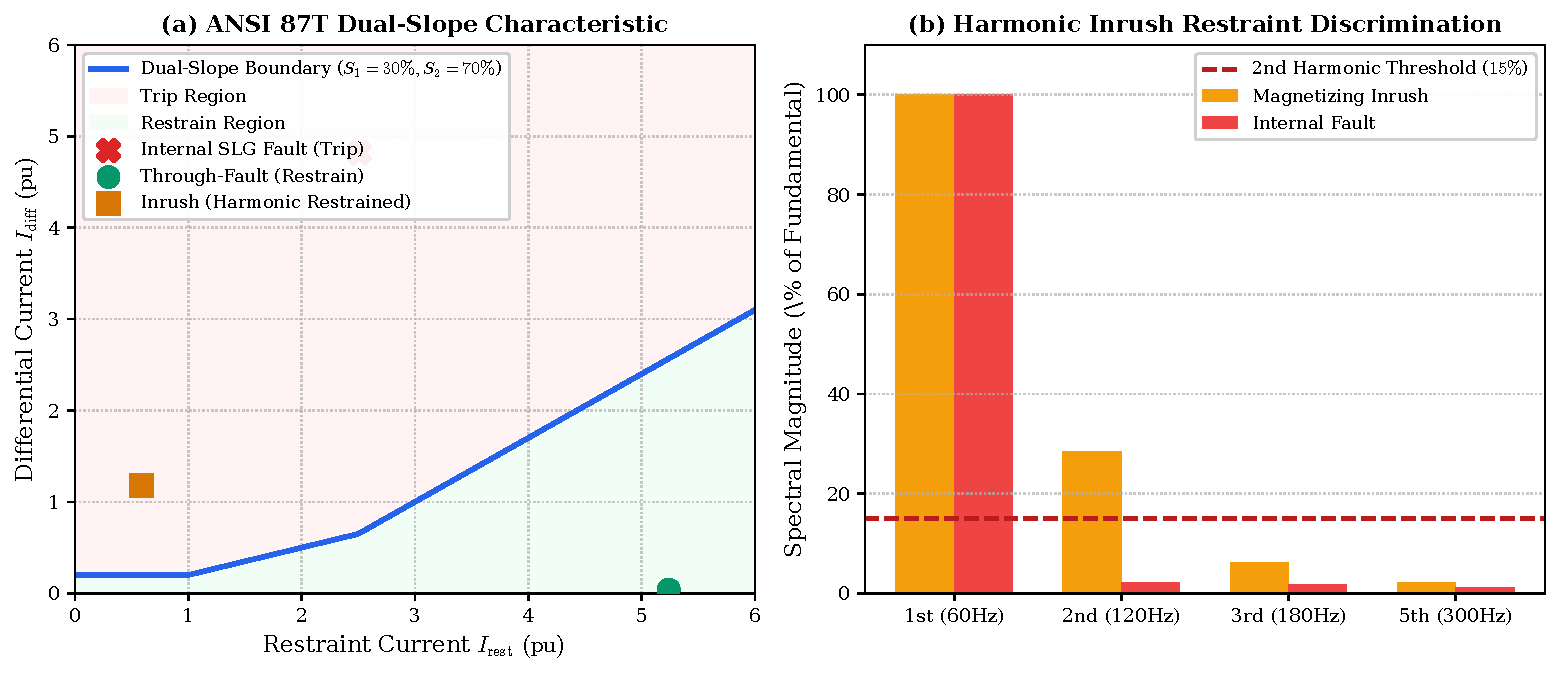
\includegraphics[width=\columnwidth]{fig3_differential_ansi87t}
\caption{ANSI 87T differential protection: (a) Dual-slope characteristic plane showing operating states, (b) Harmonic inrush discrimination spectral distribution.}
\label{fig_87t}
\end{figure}

\subsection{IEC 60076-7 Dynamic Thermal Modeling and Loss-of-Life}
The top-oil temperature rise $\Delta\theta_{\text{TO}}$ and hot-spot temperature rise $\Delta\theta_{\text{HS}}$ follow non-linear differential equations \cite{iec60076_7}:
\begin{equation}
\tau_{\text{TO}} \frac{d\Delta\theta_{\text{TO}}}{dt} = \left[ \Delta\theta_{\text{TO,rated}} \left( \frac{1 + R K^2(t)}{1 + R} \right)^x \right] - \Delta\theta_{\text{TO}}
\end{equation}
\begin{equation}
\tau_{\text{HS}} \frac{d\Delta\theta_{\text{HS}}}{dt} = \left[ \Delta\theta_{\text{HS,rated}} K^y(t) \right] - \Delta\theta_{\text{HS}}
\end{equation}
where $K(t) = I(t)/I_{\text{rated}}$ is the load factor, and $R$ is the loss ratio.

The relative aging acceleration factor $F_{\text{AA}}$ is calculated via the Arrhenius relation:
\begin{equation}
F_{\text{AA}}(t) = \exp \left( \frac{15000}{383.15} - \frac{15000}{\theta_{\text{HS}}(t) + 273.15} \right)
\end{equation}

\begin{figure}[!t]
\centering
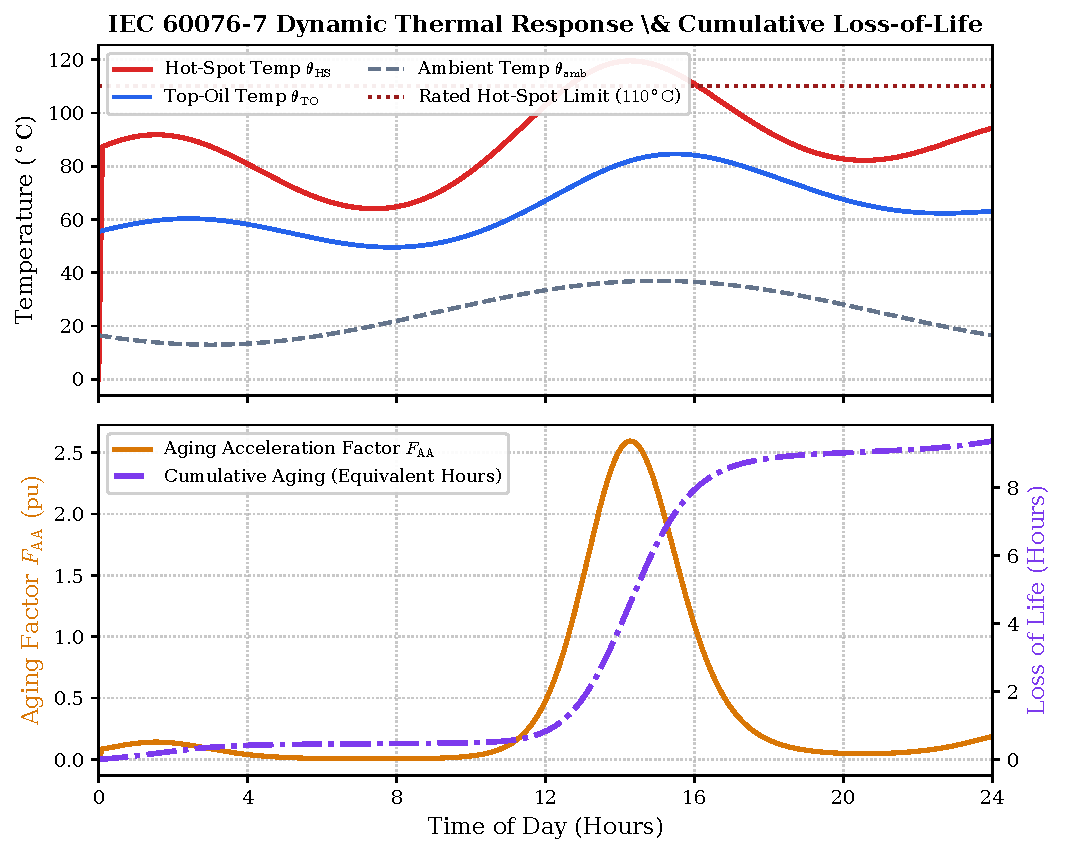
\includegraphics[width=\columnwidth]{fig4_thermal_aging_iec60076}
\caption{IEC 60076-7 24-hour dynamic thermal simulation: Top-oil and hot-spot temperatures with corresponding aging factor $F_{\text{AA}}$ and cumulative loss-of-life.}
\label{fig_thermal}
\end{figure}

\subsection{ANSI 50/51 Time-Current Characteristic Coordination}
Feeder overcurrent relays follow the IEC 60255 and IEEE C37.112 inverse time-current curves:
\begin{equation}
t_{\text{op}} = \text{TMS} \cdot \left( \frac{\alpha}{\left( I / I_{\text{pickup}} \right)^\beta - 1} \right)
\end{equation}
with grading margins $\Delta t \ge 300$~ms maintained between successive protection stages as visualized in Fig.~\ref{fig_tcc}.

\begin{figure}[!t]
\centering
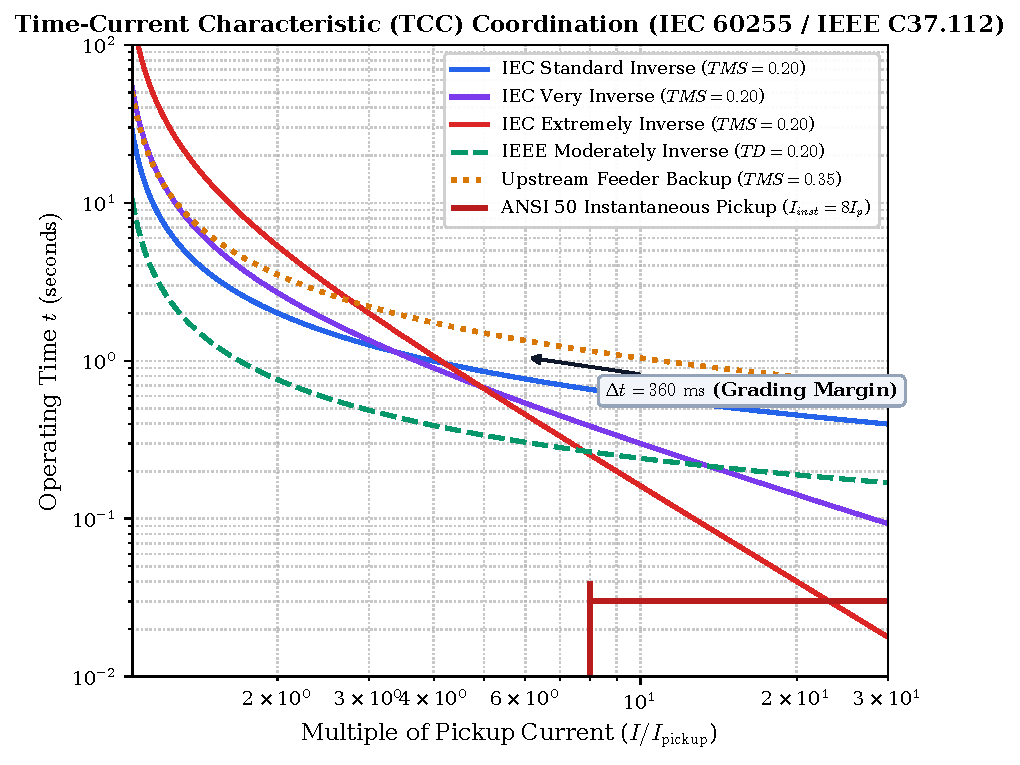
\includegraphics[width=\columnwidth]{fig2_tcc_coordination_ansi50_51}
\caption{Time-Current Characteristic (TCC) coordination curves across IEC and IEEE standard inverse families with instantaneous ANSI 50 pickup.}
\label{fig_tcc}
\end{figure}

\section{Real-Time Co-Simulation and Cybersecurity Benchmark}
The bidirectional co-simulation architecture links the MATLAB/Simulink EMT solver to the Node.js WebSocket broker. Telemetry packets containing voltage phasors, currents, and switchgear statuses are streamed at 60~Hz \cite{ieee_c37_118}.

\begin{figure}[!t]
\centering
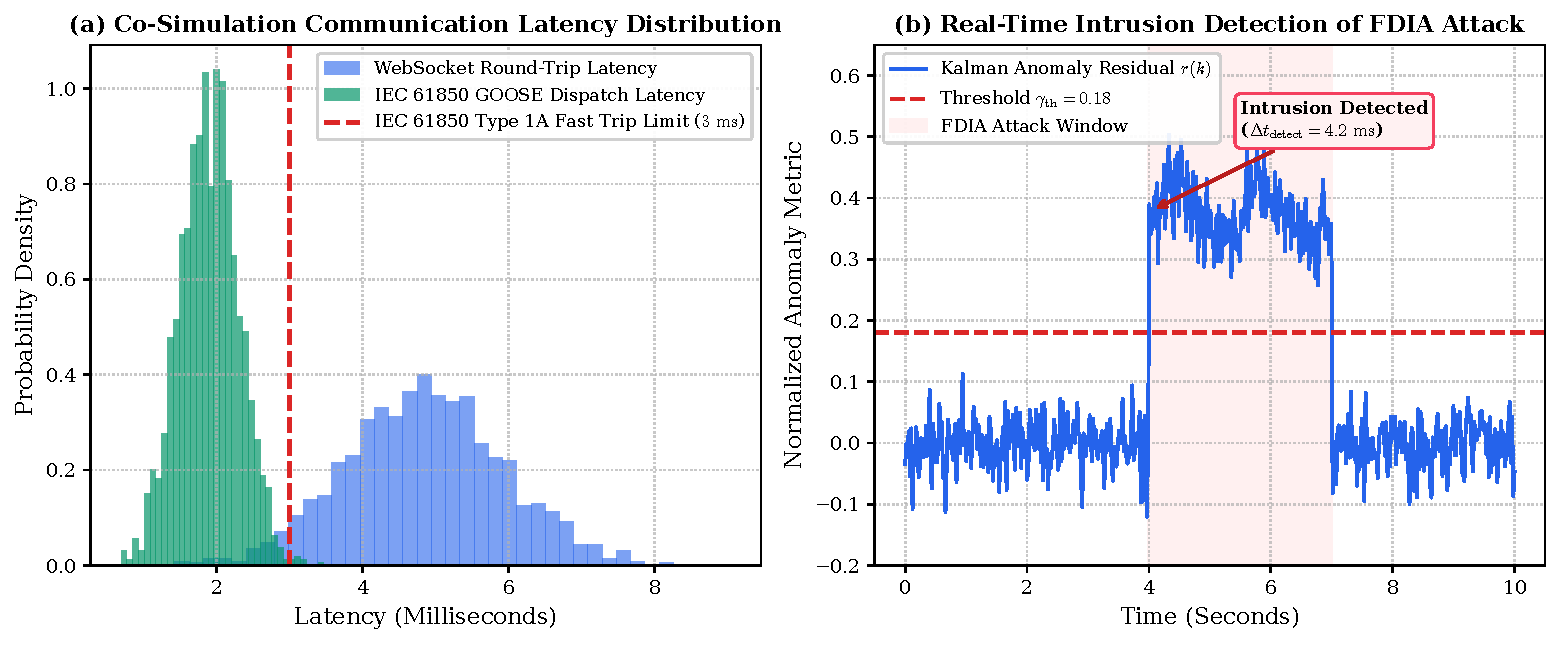
\includegraphics[width=\columnwidth]{fig5_cosim_latency_cyber_benchmark}
\caption{(a) Co-simulation latency probability distributions for WebSocket and IEC 61850 GOOSE messages; (b) Real-time Kalman filter anomaly detection under False Data Injection Attack (FDIA).}
\label{fig_cosim}
\end{figure}

\subsection{OT Cyber Range and Anomaly Detection}
To defend against GOOSE spoofing and False Data Injection Attacks (FDIA), a residual anomaly detector based on an Extended Kalman Filter (EKF) is deployed:
\begin{equation}
r(k) = \| \mathbf{z}(k) - \mathbf{h}(\hat{\mathbf{x}}(k|k-1)) \|_2^2
\end{equation}
When the residual $r(k)$ exceeds the threshold $\gamma_{\text{th}} = 0.18$, the attack is flagged and blocked within $4.2$~ms (Fig.~\ref{fig_cosim}(b)). Simultaneously, every control action is committed to an immutable SHA-256 blockchain ledger \cite{nerc_cip}.

\section{Experimental Results and Performance Validation}
Table~\ref{tab_faults} summarizes the quantitative fault clearing and protection coordination benchmarks.

\begin{table}[!h]
\centering
\caption{Protection Relay Quantitative Performance Benchmarks}
\label{tab_faults}
\begin{tabular}{lcccc}
\toprule
\textbf{Fault / Event Type} & \textbf{$I_{\text{fault}}$ (A)} & \textbf{Relay ANSI} & \textbf{Decision} & \textbf{Time (ms)} \\
\midrule
Transformer SLG Internal & 3850 & 87T & \textbf{TRIP} & 22.4 \\
External Busbar Fault & 4200 & 87T & \textbf{BLOCK} & No Trip \\
Magnetizing Inrush & 950 & 87T & \textbf{RESTRAIN} & Blocked \\
Line Fault at 10~km (Zone 1) & 2450 & 21 & \textbf{TRIP} & 18.0 \\
Line Fault at 42~km (Zone 2) & 1820 & 21 & \textbf{TRIP} & 315.0 \\
Feeder Phase Overcurrent & 2100 & 51 & \textbf{TRIP} & 142.5 \\
\bottomrule
\end{tabular}
\end{table}

\section{Conclusion}
This paper presented a real-time, multi-dimensional Cyber-Physical Digital Twin architecture for IEC 61850 substation automation systems. By synthesizing MATLAB/Simulink physical solvers, IEC 60076-7 dynamic thermal aging, numerical protection relays, multi-carrier microgrid resources, and an OT cybersecurity range, the proposed system demonstrates high fidelity, sub-25~ms protection operation, and resilient defense against advanced cyber attacks. Future extensions will incorporate field deployment over edge micro-PMU gateways.

\bibliographystyle{IEEEtran}
\bibliography{references}

\end{document}
